\documentclass[10pt,a4paper]{article}

\usepackage[margin=18mm]{geometry}
\usepackage[T1]{fontenc}
\usepackage{lmodern}
\usepackage{microtype}
\usepackage{xcolor}
\usepackage{hyperref}
\usepackage{enumitem}
\usepackage{booktabs}
\usepackage{tabularx}
\usepackage{listings}
\usepackage{tikz}
\usepackage{adjustbox}
\usetikzlibrary{arrows.meta,positioning,fit,shapes.geometric,calc}

\definecolor{tudatblue}{HTML}{176B87}
\definecolor{contractgreen}{HTML}{2E7D32}
\definecolor{jsonorange}{HTML}{C56A00}
\definecolor{runtimepurple}{HTML}{6A4C93}
\definecolor{softblue}{HTML}{EAF4F8}
\definecolor{softgreen}{HTML}{EAF5EA}
\definecolor{softorange}{HTML}{FFF2E2}
\definecolor{softpurple}{HTML}{F1ECF7}
\definecolor{softgray}{HTML}{F3F4F5}
\definecolor{codegray}{HTML}{40464D}

\hypersetup{
  colorlinks=true,
  linkcolor=tudatblue,
  urlcolor=tudatblue,
  pdftitle={TudatPy JSON Interface: Code Structure and Data Flow},
  pdfauthor={TudatPy development documentation}
}

\lstdefinestyle{pythonstyle}{
  language=Python,
  basicstyle=\ttfamily\small,
  keywordstyle=\color{tudatblue}\bfseries,
  stringstyle=\color{contractgreen},
  commentstyle=\color{codegray}\itshape,
  showstringspaces=false,
  breaklines=true,
  frame=single,
  rulecolor=\color{black!20},
  backgroundcolor=\color{softgray},
  xleftmargin=1mm,
  framexleftmargin=1mm
}

\lstdefinestyle{jsonstyle}{
  basicstyle=\ttfamily\small,
  stringstyle=\color{contractgreen},
  showstringspaces=false,
  breaklines=true,
  frame=single,
  rulecolor=\color{black!20},
  backgroundcolor=\color{softgray},
  xleftmargin=1mm,
  framexleftmargin=1mm
}

\tikzset{
  flow/.style={-{Latex[length=2.4mm]}, thick, draw=codegray},
  dataflow/.style={-{Latex[length=2.4mm]}, thick, draw=jsonorange},
  contractflow/.style={-{Latex[length=2.4mm]}, thick, dashed, draw=contractgreen},
  contextflow/.style={-{Latex[length=2.4mm]}, thick, dashed, draw=runtimepurple},
  box/.style={rounded corners=2pt, draw=codegray, thick, align=center,
              inner sep=5pt, font=\small},
  codebox/.style={box, fill=softblue, draw=tudatblue},
  contractbox/.style={box, fill=softgreen, draw=contractgreen},
  jsonbox/.style={box, fill=softorange, draw=jsonorange},
  runtimebox/.style={box, fill=softpurple, draw=runtimepurple},
  resultbox/.style={box, fill=softgray, draw=codegray}
}

\newcommand{\code}[1]{\texttt{#1}}
\newcommand{\filename}[1]{\path{#1}}

\title{\vspace{-12mm}\textbf{TudatPy JSON Interface}\\[1mm]
\large Code Structure, Contract Semantics, and Data Flow}
\author{Architecture report for the contract-driven settings interface}
\date{\today}

\begin{document}
\maketitle
\vspace{-4mm}

\begin{abstract}
The JSON interface is a settings-construction layer. JSON contracts define the
permitted data model; the generic loader validates JSON values against those
contracts and calls the same public TudatPy settings factories used by ordinary
Python applications. It does not serialize runtime objects, propagate dynamics,
or maintain a second hand-written implementation of each settings family. This
report documents the implemented code structure, the flow of linked JSON data,
and the end-to-end perturbed-satellite regression test.
\end{abstract}

\section{Architectural rules}

The implementation follows five rules:

\begin{enumerate}[leftmargin=7mm,itemsep=1.5mm]
  \item \textbf{Contracts are authoritative.} Factory names, argument names,
        types, optional defaults, and temporarily unsupported inputs live in JSON
        contract files.
  \item \textbf{The loader is generic.} Nested settings are recognized from
        dotted contract types and recursively constructed without module-specific
        conversion code.
  \item \textbf{Factories are public TudatPy API.} A JSON factory name maps to a
        callable exposed by an identifiable \code{environment\_setup} or
        \code{propagation\_setup} module.
  \item \textbf{JSON contains settings data only.} Live runtime objects such as
        \code{SystemOfBodies} are passed as context after environment creation.
  \item \textbf{References compose files.} An object containing only
        \code{"\$ref"} is replaced by the referenced JSON value, with paths
        resolved relative to the file containing the reference.
\end{enumerate}

\section{Code and file structure}

\begin{figure}[ht]
\centering
\begin{adjustbox}{max width=\textwidth}
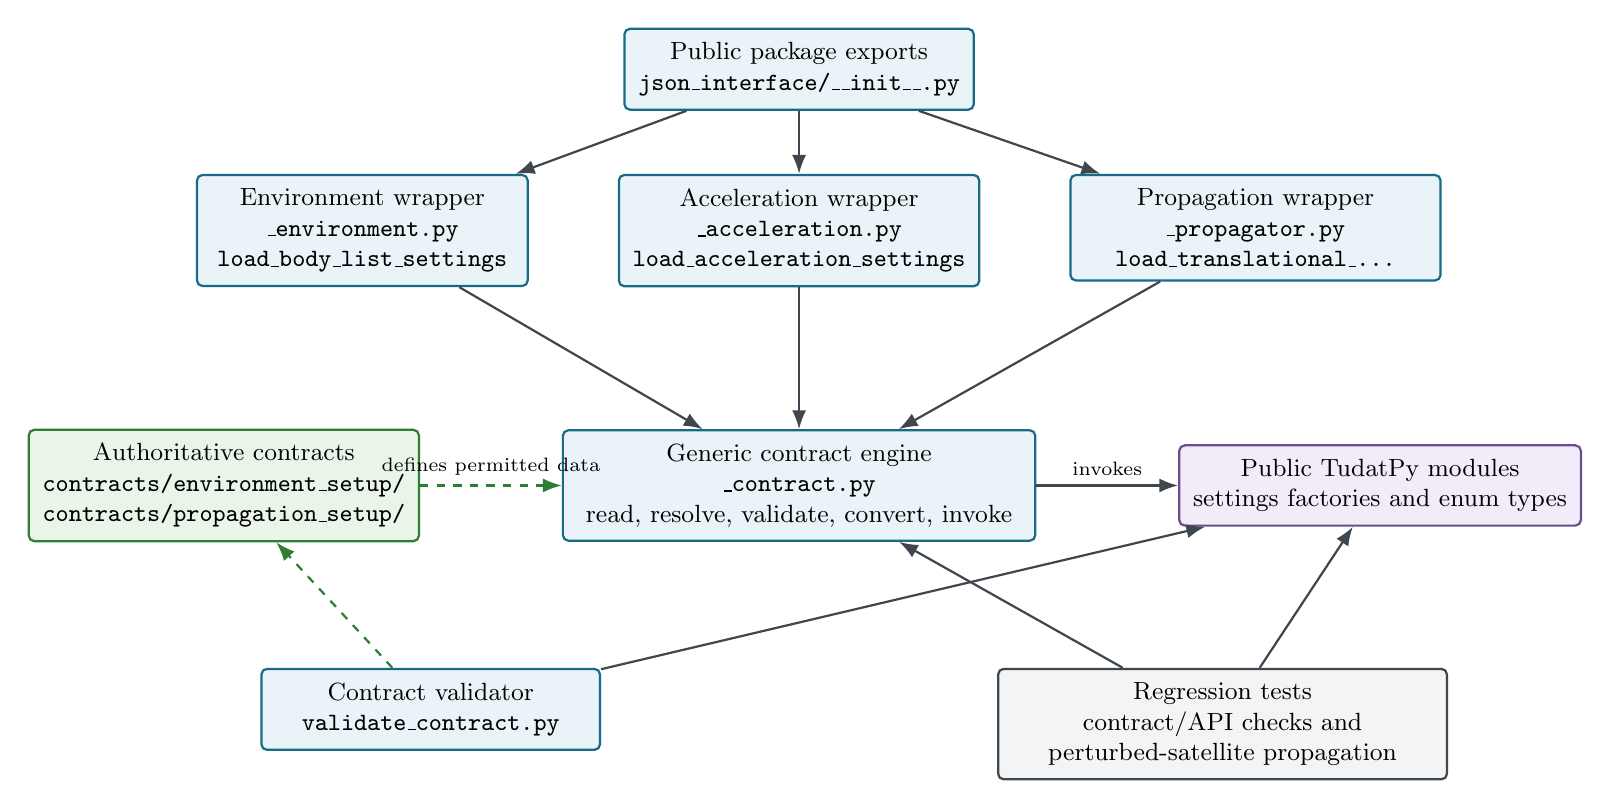
\begin{tikzpicture}[node distance=8mm and 12mm]
  \node[codebox, minimum width=42mm] (public) {Public package exports\\\code{json\_interface/\_\_init\_\_.py}};

  \node[codebox, below left=of public, minimum width=42mm] (env) {Environment wrapper\\\code{\_environment.py}\\\code{load\_body\_list\_settings}};
  \node[codebox, below=of public, minimum width=42mm] (acc) {Acceleration wrapper\\\code{\_acceleration.py}\\\code{load\_acceleration\_settings}};
  \node[codebox, below right=of public, minimum width=47mm] (prop) {Propagation wrapper\\\code{\_propagator.py}\\\code{load\_translational\_...}};

  \node[codebox, below=18mm of acc, minimum width=60mm] (engine) {Generic contract engine\\\code{\_contract.py}\\read, resolve, validate, convert, invoke};
  \node[contractbox, left=18mm of engine, minimum width=45mm] (contracts) {Authoritative contracts\\\code{contracts/environment\_setup/}\\\code{contracts/propagation\_setup/}};
  \node[runtimebox, right=18mm of engine, minimum width=49mm] (api) {Public TudatPy modules\\settings factories and enum types};

  \node[codebox, below left=16mm and -5mm of engine, minimum width=43mm] (validator) {Contract validator\\\code{validate\_contract.py}};
  \node[resultbox, below right=16mm and -5mm of engine, minimum width=57mm] (tests) {Regression tests\\contract/API checks and\\perturbed-satellite propagation};

  \draw[flow] (public) -- (env);
  \draw[flow] (public) -- (acc);
  \draw[flow] (public) -- (prop);
  \draw[flow] (env) -- (engine);
  \draw[flow] (acc) -- (engine);
  \draw[flow] (prop) -- (engine);
  \draw[contractflow] (contracts) -- node[above,font=\scriptsize] {defines permitted data} (engine);
  \draw[flow] (engine) -- node[above,font=\scriptsize] {invokes} (api);
  \draw[contractflow] (validator) -- (contracts);
  \draw[flow] (validator) -- (api);
  \draw[flow] (tests) -- (engine);
  \draw[flow] (tests) -- (api);
\end{tikzpicture}
\end{adjustbox}
\caption{Implemented module structure. Solid arrows represent Python calls;
dashed green arrows represent contract-governed validation.}
\end{figure}

\subsection{Responsibilities}

\noindent\begin{tabularx}{\textwidth}{@{}>{\raggedright\arraybackslash}p{38mm}>{\raggedright\arraybackslash}X@{}}
\toprule
\textbf{Component} & \textbf{Responsibility} \\
\midrule
\code{\_contract.py} & Reads JSON, resolves references, parses type expressions,
validates defaults and factory signatures, converts values, and invokes factories. \\
\code{\_environment.py} & Extracts the global frame and injects it as context when
creating the linked per-body settings, then returns \code{BodyListSettings}. \\
\code{\_acceleration.py} & Selects the acceleration contract for the standard nested
body/exerting-body acceleration-settings mapping. \\
\code{\_propagator.py} & Injects the live body system so the public composition
factory can create acceleration models from JSON acceleration settings. \\
\code{validate\_contract.py} & Compares arbitrary contracts, or all packaged
contracts, with the first exposed signatures of their public TudatPy factories. \\
\code{contracts/} & Shared data-model definitions. Editing a contract changes what
the generic loader accepts; no parallel factory-specific loader table is required. \\
\bottomrule
\end{tabularx}

\section{Generic settings-construction pipeline}

For every loader call, the same pipeline is used:

\begin{enumerate}[leftmargin=7mm,itemsep=1.5mm]
  \item \code{read\_json\_object} decodes the root file and recursively replaces
        relative \code{\$ref} objects.
  \item \code{load\_contract} validates the contract structure, all type
        expressions, optional defaults, unsupported declarations, and factory
        existence.
  \item \code{\_convert\_settings\_tree} preserves structural dictionaries while
        recognizing one-key factory definitions at the leaves.
  \item \code{create\_settings\_object} checks missing, unknown, and unsupported
        arguments; merges operational defaults; and converts every supported value.
  \item The selected callable is retrieved from the public TudatPy module and
        invoked with converted JSON arguments plus any explicitly supplied runtime
        context.
\end{enumerate}

\subsection{Contract entry semantics}

\begin{lstlisting}[style=jsonstyle]
"spherical_harmonic_gravity": {
  "properties": {
    "maximum_degree": "int",
    "maximum_order": "int"
  }
}
\end{lstlisting}

All properties are required unless their name appears in \code{optional}. A
finite optional value is passed explicitly to the Tudat factory; a
\code{null} default delegates to the factory default when JSON cannot represent
that default reliably. An input in \code{unsupported} remains visible in the
shared contract, but cannot be supplied. If it is required, that factory cannot
yet be constructed from JSON; if it is optional and omitted, Tudat uses its own
default.

\section{End-to-end data flow}

The perturbed-satellite test has two top-level settings inputs. Both can include
arbitrarily nested relative references, but the Python test loads only these two
root documents.

\begin{figure}[p]
\centering
\begin{adjustbox}{max width=\textwidth, max totalheight=0.88\textheight}
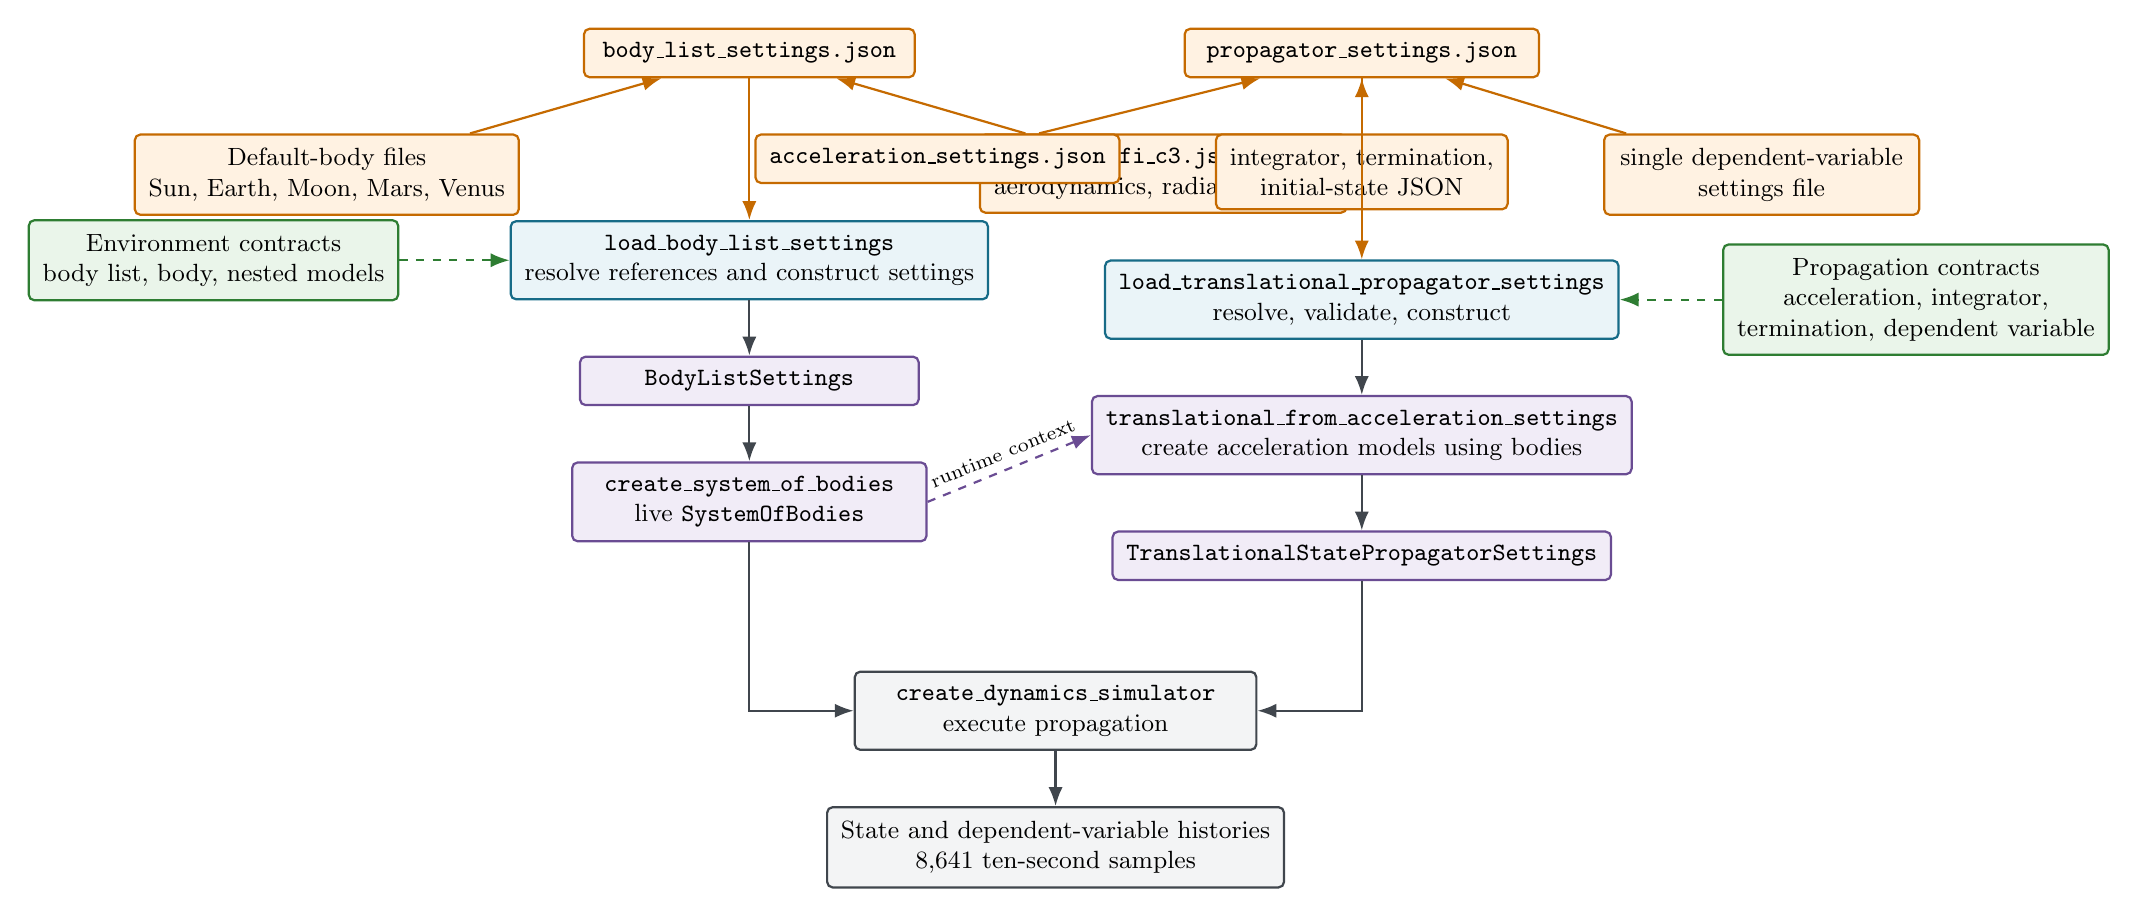
\begin{tikzpicture}[node distance=7mm and 8mm]
  \node[jsonbox, minimum width=42mm] (bodyroot) {\code{body\_list\_settings.json}};
  \node[jsonbox, below left=of bodyroot, minimum width=34mm] (defaults) {Default-body files\\Sun, Earth, Moon, Mars, Venus};
  \node[jsonbox, below right=of bodyroot, minimum width=38mm] (delfi) {\code{delfi\_c3.json}\\aerodynamics, radiation, mass};

  \node[codebox, below=18mm of bodyroot, minimum width=48mm] (bodyloader) {\code{load\_body\_list\_settings}\\resolve references and construct settings};
  \node[contractbox, left=14mm of bodyloader, minimum width=42mm] (envcontracts) {Environment contracts\\body list, body, nested models};
  \node[runtimebox, below=of bodyloader, minimum width=43mm] (bodysettings) {\code{BodyListSettings}};
  \node[runtimebox, below=of bodysettings, minimum width=45mm] (bodies) {\code{create\_system\_of\_bodies}\\live \code{SystemOfBodies}};

  \node[jsonbox, right=34mm of bodyroot, minimum width=45mm] (proproot) {\code{propagator\_settings.json}};
  \node[jsonbox, below left=of proproot, minimum width=36mm] (accjson) {\code{acceleration\_settings.json}};
  \node[jsonbox, below=of proproot, minimum width=37mm] (numjson) {integrator, termination,\\initial-state JSON};
  \node[jsonbox, below right=of proproot, minimum width=40mm] (depjson) {single dependent-variable\\settings file};

  \node[codebox, below=23mm of proproot, minimum width=53mm] (proploader) {\code{load\_translational\_propagator\_settings}\\resolve, validate, construct};
  \node[contractbox, right=13mm of proploader, minimum width=44mm] (propcontracts) {Propagation contracts\\acceleration, integrator,\\termination, dependent variable};
  \node[runtimebox, below=of proploader, minimum width=55mm] (compose) {\code{translational\_from\_acceleration\_settings}\\create acceleration models using bodies};
  \node[runtimebox, below=of compose, minimum width=50mm] (propsettings) {\code{TranslationalStatePropagatorSettings}};

  \node[resultbox, below=18mm of $(bodies)!0.5!(propsettings)$, minimum width=51mm] (sim) {\code{create\_dynamics\_simulator}\\execute propagation};
  \node[resultbox, below=of sim, minimum width=48mm] (results) {State and dependent-variable histories\\8,641 ten-second samples};

  \draw[dataflow] (defaults) -- (bodyroot);
  \draw[dataflow] (delfi) -- (bodyroot);
  \draw[dataflow] (bodyroot) -- (bodyloader);
  \draw[contractflow] (envcontracts) -- (bodyloader);
  \draw[flow] (bodyloader) -- (bodysettings);
  \draw[flow] (bodysettings) -- (bodies);

  \draw[dataflow] (accjson) -- (proproot);
  \draw[dataflow] (numjson) -- (proproot);
  \draw[dataflow] (depjson) -- (proproot);
  \draw[dataflow] (proproot) -- (proploader);
  \draw[contractflow] (propcontracts) -- (proploader);
  \draw[flow] (proploader) -- (compose);
  \draw[contextflow] (bodies.east) -- node[above,sloped,font=\scriptsize] {runtime context} (compose.west);
  \draw[flow] (compose) -- (propsettings);
  \draw[flow] (bodies) |- (sim);
  \draw[flow] (propsettings) |- (sim);
  \draw[flow] (sim) -- (results);
\end{tikzpicture}
\end{adjustbox}
\caption{Data flow in the JSON-only perturbed-satellite test. Orange arrows are
JSON/reference flow, dashed green arrows are contract validation, dashed purple
is the live body context, and solid dark arrows are object/runtime flow.}
\end{figure}

\clearpage
\section{The explanatory end-to-end test}

The test is located at
\code{tests/test\_tudatpy/json\_interface/perturbed\_satellite\_orbit/}.
Its Python body deliberately contains no direct settings-factory calls:

\begin{lstlisting}[style=pythonstyle]
def test_perturbed_satellite_orbit_from_json():
    # Runtime initialization, not settings construction.
    spice.load_standard_kernels()

    body_list_settings = load_body_list_settings(
        settings_directory / "body_list_settings.json"
    )
    bodies = environment_setup.create_system_of_bodies(body_list_settings)

    propagator_settings = load_translational_propagator_settings(
        settings_directory / "propagator_settings.json", bodies
    )

    dynamics_simulator = simulator.create_dynamics_simulator(
        bodies, propagator_settings
    )

    assert len(dynamics_simulator.propagation_results.state_history) == 8641
\end{lstlisting}

\subsection{Environment input}

\code{body\_list\_settings.json} declares the Earth-centered J2000 global frame
and references six per-body files. The five celestial bodies request Tudat
defaults. \code{body\_settings/delfi\_c3.json} contains all Delfi-C3 environment
properties in one place:

\begin{itemize}[leftmargin=7mm,itemsep=1mm]
  \item constant aerodynamic coefficients with reference area
        $0.035\,\mathrm{m^2}$ and force coefficients $[1.2,0,0]$;
  \item a cannonball radiation-pressure target with coefficient $1.2$ and Earth
        occulting the Sun;
  \item constant rigid-body properties with mass $2.2\,\mathrm{kg}$.
\end{itemize}

The environment wrapper propagates the root global frame into the construction
of every default body. It returns \code{BodyListSettings}; ordinary TudatPy then
creates the live body system.

\subsection{Propagation input}

\code{propagator\_settings.json} references separate files for:

\noindent\begin{tabularx}{\textwidth}{@{}>{\raggedright\arraybackslash}p{58mm}>{\raggedright\arraybackslash}X@{}}
\toprule
\textbf{File} & \textbf{Contents} \\
\midrule
\filename{acceleration_settings.json} & Spherical-harmonic Earth gravity to degree
and order 5, Earth aerodynamics, Sun radiation pressure, and point-mass gravity
from Sun, Moon, Mars, and Venus. \\
\filename{integrator_settings.json} & Fixed-step RK4 with a ten-second step. \\
\filename{termination_settings.json} & Time termination at the end of the one-day
interval. \\
\filename{initial_state_from_tle.json} & Cartesian state derived from the TLE used
by the ordinary perturbed-satellite example. \\
\filename{dependent_variable_settings.json} & Total acceleration, Keplerian state,
latitude, longitude, and the norms of each individual acceleration contribution. \\
\bottomrule
\end{tabularx}

The propagation wrapper supplies the live body system only as runtime context.
The public \filename{translational_from_acceleration_settings} factory creates
acceleration models and then constructs ordinary translational propagator
settings. The simulator call is therefore unchanged from a normal TudatPy
application.

\subsection{What the assertion proves}

The expected 8,641 samples follow from an inclusive one-day interval sampled at
ten-second integration steps:
\[
  \frac{86{,}400\ \mathrm{s}}{10\ \mathrm{s}} + 1 = 8{,}641.
\]
Reaching this assertion demonstrates that all linked files were resolved, every
nested settings definition passed its contract, public Tudat factories created
the environment and propagation settings, acceleration models were composed with
the runtime bodies, and the resulting settings supported a complete propagation.

\section{Validation and failure boundaries}

The regression suite separates structural correctness from end-to-end execution:

\begin{enumerate}[leftmargin=7mm,itemsep=1.5mm]
  \item \textbf{Contract/API parity:} every contract factory exists and its
        required/optional argument names match the first public signature.
  \item \textbf{Documentation parity:} every contracted factory is present in
        the generated API documentation sources.
  \item \textbf{Type enforcement:} wrong scalar types, missing inputs, unknown
        inputs, unknown factories, and non-finite numbers are rejected before the
        factory call.
  \item \textbf{Default semantics:} finite contract defaults are operational;
        null and optional unsupported inputs delegate to Tudat defaults.
  \item \textbf{Reference semantics:} relative references work recursively and
        circular references are rejected.
  \item \textbf{Runtime composition:} body settings create the system of bodies,
        and those bodies are injected only where acceleration-model construction
        requires them.
  \item \textbf{Execution:} the perturbed-satellite test completes the one-day
        propagation and checks the full sample count.
\end{enumerate}

\section{Extension path}

For an ordinary additional \code{environment\_setup} or
\code{propagation\_setup} settings family, the intended extension is:

\begin{enumerate}[leftmargin=7mm,itemsep=1.5mm]
  \item add or update its authoritative JSON contract;
  \item ensure each factory is public, documented, and has a finite named-input
        interface;
  \item use dotted property types to connect settings families;
  \item mark inputs outside the supported settings layer explicitly as
        \code{unsupported};
  \item run the generic validator and relevant end-to-end tests.
\end{enumerate}

No new conversion dispatch table is required. A thin wrapper is justified only
when the outer document has a domain-specific shape or construction requires a
live runtime object that cannot belong in JSON.

\end{document}
